\mchapter{روش پیشنهادی}
\section{پردازش و جمع آوری داده}
برای آموزش مدل، به داده‌های برچسب‌خورده نیاز بود. در این پروژه از داده‌های موجود در لینک زیر استفاده شده است:
\begin{latin}
	\url{https://github.com/liyichen1234/HMML}
\end{latin}
این مجموعه داده‌ها شامل ۳۹۶۴۷ پروژه جاوا می‌باشد که هر پروژه حاوی ۲ تا ۱۰ فایل کد جاوا است. برای هر پروژه بین یک تا پنج برچسب بوی کد تخصیص داده شده است.

در ابتدا، تمامی فایل‌های کد مرتبط با هر پروژه ادغام شدند و سپس برچسب‌های اختصاص داده شده به هر پروژه به‌صورت یک رشته ترکیبی از برچسب‌ها تبدیل شدند. در نهایت، یک جدول با فرمت فایل \lr{csv} ایجاد شد. در ستون اول این جدول، آدرس فایل ادغام‌شده پروژه‌ها و در ستون دوم، نام بوی کدهای مربوط به آن پروژه قرار گرفت.

برای آموزش مدل، هر فایل کد باید با استفاده از آدرس موجود در جدول واژه‌بندی\LTRfootnote{tokenize} شده و در کارت گرافیک بارگذاری شود. همچنین، برچسب‌های هر پروژه به صورت یک آرایه به طول ۲۸ تبدیل می‌شوند که در آن هر خانه با مقدار ۰ یا ۱ مشخص می‌کند که آیا بوی کد مورد نظر در آن پروژه جاوا وجود دارد یا خیر.\cite{BOGATINOVSKI2022117215}
\section{تعریف مدل}
در یادگیری عمیق مدل به عنوان ساختار محاسباتی اصلی عمل می‌کند که ورودی‌ها را بر اساس داده‌های مشاهده شده به خروجی‌ها نگاشت می‌کند. مدل با استفاده از یک مجموعه داده آموزش می‌بیند و الگوها، روابط و قوانینی را یاد می‌گیرد که می‌تواند برای پیش‌بینی داده‌های جدید و نادیده گرفته‌شده تعمیم یابد. مدل‌های مدرن، به‌ویژه آن‌هایی که بر روی معماری‌های یادگیری عمیق مانند مبدلها ساخته شده‌اند، در شناسایی الگوهای پیچیده در داده‌ها بسیار قدرتمند هستند. با این حال، اغلب نیاز به سفارشی‌سازی و توسعه دارند تا برای وظایف خاص مناسب شوند. این مقاله به فرآیند بارگذاری یک مدل از پیش‌آموزش‌دیده، به‌ویژه یک مدل زبان بزرگ \lr{(LLM)}، و سپس تطبیق آن برای یک وظیفه طبقه‌بندی چند‌برچسبی از طریق اتصال لایه نهایی آن به یک شبکه عصبی چندلایه\LTRfootnote{Multi Layer Perceptron} برای طبقه‌بندی در ۲۸ برچسب مختلف می‌پردازد.\cite{Zhang2022code}
\subsection{بارگذاری مدل از پیش‌آموزش‌دیده}

یک مدل زبان بزرگ، مانند \lr{GPT} یا \lr{LLama}، معمولاً بر روی حجم عظیمی از داده‌های متنی از پیش‌آموزش دیده تا بتواند زبان طبیعی را درک و تولید کند. این مدل‌ها با معماری‌های عمیق و چندلایه طراحی شده‌اند که می‌توانند ویژگی‌های پیچیده زبان‌شناسی را شناسایی کنند. فاز پیش‌آموزش به مدل اجازه می‌دهد تا وظایف مختلف زبانی مانند طبقه‌بندی متن، تحلیل احساسات و ترجمه زبان را با استفاده از بازنمایی‌های داخلی زبان یاد بگیرد.
\\
برای شروع، مدل از پیش‌آموزش‌دیده در محیط محاسباتی بارگذاری می‌شود. این مرحله شامل وارد کردن معماری مدل و وزن‌های یادگرفته‌شده آن است. فرآیند بارگذاری می‌تواند با استفاده از فریم‌ورک‌های یادگیری عمیق محبوب مانند \lr{TensorFlow} یا \lr{PyTorch} انجام شود که \lr{API} هایی برای بارگذاری آسان این مدل‌های از پیش‌آموزش‌دیده ارائه می‌دهند.
به عنوان مثال، در \lr{PyTorch}، این کار با یک فرمان ساده مانند \lr{`model = AutoModel.from\_pretrained('model\_name')`} انجام می‌شود، که در آن \lr{`model\_name`} مدل پیش‌آموزش‌دیده مورد نظر را مشخص می‌کند.
\\
پس از بارگذاری، مدل زبان بزرگ می‌تواند برای وظایف خاص تنظیم یا تطبیق داده شود. اگرچه مدل قبلاً قادر به درک و تولید زبان است، اما ممکن است به طور مستقیم برای وظایفی که نیاز به خروجی‌های ساختاریافته دارند، مانند طبقه‌بندی چند‌برچسبی، مناسب نباشد. بنابراین، باید لایه‌های اضافی یا مولفه‌های دیگر اضافه شود.
\subsection{اتصال مدل زبان بزرگ به یک شبکه عصبی چندلایه}

برای وظیفه مورد نظر طبقه‌بندی چند‌برچسبی با ۲۸ برچسب لایه نهایی مدل زبان بزرگ باید تطبیق داده شود. به طور معمول، خروجی یک مدل زبان بزرگ یک بازنمایی با ابعاد بالا از متن ورودی است که اغلب به عنوان "وضعیت پنهان" یا "تعبیر" شناخته می‌شود. این بازنمایی شامل اطلاعات غنی است اما به طور مستقیم برای وظایف طبقه‌بندی قابل تفسیر نیست.

برای تبدیل این بازنمایی به مجموعه‌ای از طبقه‌بندی‌ها، وضعیت پنهان نهایی مدل زبان بزرگ به یک شبکه عصبی چندلایه متصل می‌شود. شبکه عصبی چندلایه یک شبکه عصبی ساده اما قدرتمند است که از یک یا چند لایه کاملاً متصل تشکیل شده است. شبکه عصبی چندلایه بازنمایی با ابعاد بالا از مدل زبان بزرگ را دریافت کرده و آن را برای تولید خروجی مطلوب پردازش می‌کند.

در اینجا نحوه انجام این فرآیند آمده است:
\begin{enumerate}
	\item
	      استخراج بازنمایی: خروجی مدل زبان بزرگ، که اغلب یک بردار با هزاران بعد است، به عنوان ورودی به شبکه عصبی چندلایه ارسال می‌شود. این بازنمایی جوهره متن ورودی را به شکلی که شبکه عصبی چندلایه بتواند پردازش کند، ثبت می‌کند.
	\item
	      طراحی شبکه عصبی چندلایه: شبکه عصبی چندلایه با یک یا چند لایه طراحی شده است. لایه نهایی شبکه عصبی چندلایه باید دارای ۲۸ نرون (یا گره) باشد که با ۲۸ برچسب در وظیفه طبقه‌بندی مطابقت دارد. هر نرون در لایه نهایی یک مقدار را خروجی می‌دهد که نمایانگر احتمال تعلق ورودی به آن برچسب خاص است. این خروجی‌ها معمولاً با استفاده از یک تابع فعال‌سازی \lr{sigmoid} تفسیر می‌شوند.

	\item
	      خروجی چند‌برچسبی: برخلاف وظایف طبقه‌بندی سنتی که در آن تنها یک برچسب پیش‌بینی می‌شود، طبقه‌بندی چند‌برچسبی امکان فعال بودن چندین برچسب به طور همزمان را فراهم می‌کند. لایه خروجی شبکه عصبی چندلایه به گونه‌ای طراحی شده است که با اعمال تابع \lr{sigmoid} به هر یک از ۲۸ خروجی، این کار را انجام دهد. این تابع هر خروجی را به احتمالی بین 0 و 1 نگاشت می‌کند، که در آن یک آستانه (معمولاً \lr{0.5}) برای تعیین فعال بودن یا نبودن هر برچسب اعمال می‌شود.

	\item
	      آموزش مدل توسعه‌یافته: کل مدل شامل مدل زبان بزرگ و شبکه عصبی چندلایه متصل شده باید بر روی یک مجموعه داده چندبرچسبی آموزش داده شود. در این فاز، مدل یاد می‌گیرد که پارامترهای خود را، به ویژه آن‌هایی که در شبکه عصبی چندلایه هستند، تنظیم کند تا اختلاف بین پیش‌بینی‌های خود و برچسب‌های واقعی در مجموعه داده را به حداقل برساند. این کار معمولاً با استفاده از یک تابع زیان طراحی شده برای طبقه‌بندی چندبرچسبی، مانند آنتروپی\LTRfootnote{Entropy} متقاطع باینری، انجام می‌شود.
\end{enumerate}

\begin{figure}[H]
	\centering
	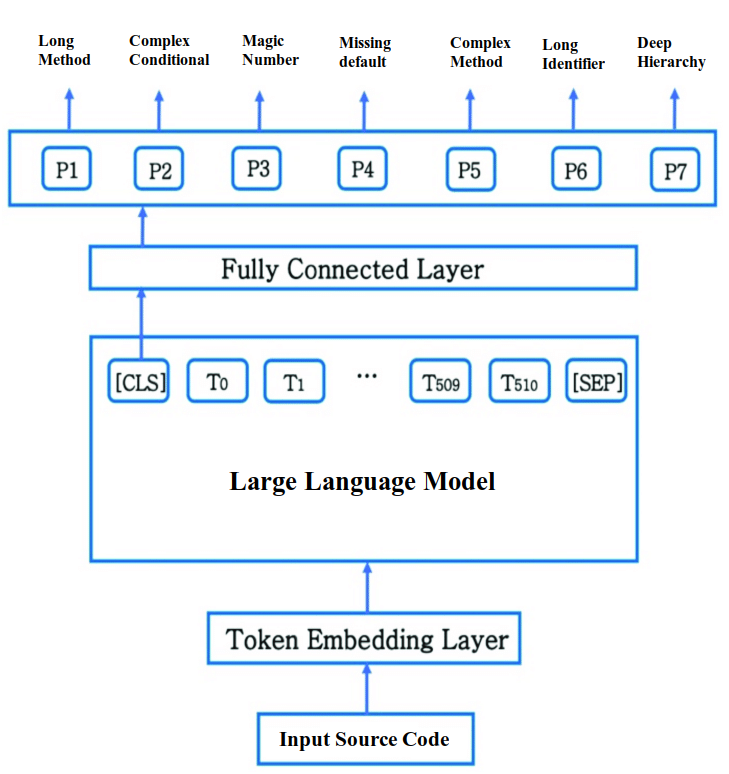
\includegraphics[width=0.8\textwidth]{figures/finetune.png}
	\caption{نحوه بهبود دادن مدل}
	\label{fig:finetune}
\end{figure}
\clearpage
همانطور که در شکل \ref{fig:finetune} ملاحظه میکنید،
با بارگذاری یک مدل زبان بزرگ از پیش‌آموزش‌دیده و اتصال لایه نهایی آن به یک شبکه عصبی چندلایه، می‌توانیم مدل را به طور مؤثری برای وظایف پیچیده‌ای مانند طبقه‌بندی چند‌برچسبی با ۲۸ برچسب تطبیق دهیم. این رویکرد از توانایی‌های قدرتمند درک زبان مدل‌های زبان بزرگ بهره می‌برد و در عین حال آن‌ها را برای مدیریت خروجی‌های ساختاریافته خاص گسترش می‌دهد. نتیجه یک مدل بسیار تخصصی است که می‌تواند چندین برچسب را برای یک ورودی پیش‌بینی کند و آن را به یک ابزار همه‌کاره برای وظایف مختلف پردازش زبان طبیعی تبدیل می‌کند.\cite{j2024finetuningllmenterprise}

\section{آموزش مدل}

توسعه و بهینه‌سازی مدل‌های زبانی به‌طور فزاینده‌ای پیچیده شده است. یکی از دستاوردهای برجسته در این مسیر، ظهور مدل‌های زبانی بزرگ \lr{(LLMs)} است که توانایی فوق‌العاده‌ای در درک و تولید متن شبیه به انسان دارند. با این حال، آموزش این مدل‌ها چالش‌های زیادی را به همراه دارد، به‌ویژه از نظر نیاز به منابع محاسباتی و کارایی در بهینه‌سازی. در میان روش‌های مختلفی که برای مقابله با این چالش‌ها توسعه یافته‌اند،\lr{QLoRA}\LTRfootnote{Quantized Low-Ranked Adaptation of Language Models} (تطبیق ماتریس‌های کم‌رتبه با استفاده از فشرده‌سازی\LTRfootnote{Quantize}) به‌عنوان یک رویکرد امیدوارکننده مطرح شده است. این مقاله به مفهوم تعریف مدل می‌پردازد و جزئیات آموزش مدل‌های زبانی بزرگ با استفاده از \lr{QLoRA} را بررسی می‌کند.

\subsection{چالش‌های آموزش مدل‌های زبانی بزرگ}

آموزش مدل‌های زبانی بزرگ یک وظیفه پیچیده است که نیازمند قدرت محاسباتی، حافظه و داده‌های عظیم است. با افزایش اندازه این مدل‌ها، نیاز به منابع سخت‌افزاری نیز افزایش می‌یابد و آموزش آن‌ها بر روی سخت‌افزارهای استاندارد دشوار می‌شود. علاوه بر این، بهینه‌سازی این مدل‌ها برای وظایف خاص یا حوزه‌های خاص به تلاش محاسباتی بیشتری نیاز دارد که اغلب به هزینه‌های بالایی منجر می‌شود.
\\
یکی از چالش‌های کلیدی در آموزش مدل‌های زبانی بزرگ، تعادل بین اندازه مدل و کارایی محاسباتی است. مدل‌های بزرگ‌تر معمولاً عملکرد بهتری دارند اما در عین حال منابع بیشتری را مصرف می‌کنند، که باعث می‌شود پیاده‌سازی آن‌ها در محیط‌هایی با منابع محدود دشوار شود. برای مقابله با این چالش‌ها، محققان روش‌های مختلفی را توسعه داده‌اند، از جمله فشرده‌سازی و تطبیق ماتریس‌های کم‌رتبه، که هدف آن‌ها کاهش بار محاسباتی بدون کاهش قابل توجه عملکرد مدل است.

\subsection{معرفی \lr{QLoRA}}

\lr{QLoRA} (تطبیق ماتریس‌های کم‌رتبه با استفاده از فشرده‌سازی) یک روش است که برای بهبود کارایی آموزش مدل‌های زبانی بزرگ با ترکیب دو مفهوم قدرتمند طراحی شده است: فشرده‌سازی و تطبیق ماتریس‌های کم‌رتبه.
\begin{enumerate}
	\item
	      فشرده‌سازی: این فرآیند شامل کاهش دقت وزن‌های مدل از فرمت‌های با دقت بالا (مانند فلوتینگ‌پوینت ۳۲ بیتی) به فرمت‌های با دقت پایین‌تر (مانند اعداد صحیح ۸ بیتی) است. فشرده‌سازی به‌طور قابل توجهی حجم حافظه و نیازهای محاسباتی مدل را کاهش می‌دهد و به آن امکان می‌دهد تا به‌طور کارآمدتری بر روی سخت‌افزارهای کم‌قدرت اجرا شود. در حالی که فشرده‌سازی ممکن است منجر به کاهش جزئی در دقت مدل شود، این کاهش در مقایسه با مزایای به‌دست‌آمده از نظر کارایی منابع اغلب ناچیز است.
	\item
	      تطبیق ماتریس‌های کم‌رتبه: این روش شامل تقریب ماتریس‌های وزن مدل به‌عنوان حاصل‌ضرب دو ماتریس کوچک‌تر با رتبه کمتر است. با کاهش رتبه، تعداد پارامترها به‌طور قابل توجهی کاهش می‌یابد که به نوبه خود بار محاسباتی در طول آموزش را کاهش می‌دهد. تطبیق ماتریس‌های کم‌رتبه امکان بهینه‌سازی کارآمد مدل‌های زبانی بزرگ را فراهم می‌کند و بر روی پارامترهای با بیشترین اطلاعات تمرکز می‌کند، در نتیجه سرعت آموزش را افزایش داده و مصرف منابع را کاهش می‌دهد.
\end{enumerate}

\subsection{آموزش مدل‌های زبانی بزرگ با \lr{QLoRA}}

\lr{QLoRA} این دو روش را ترکیب می‌کند تا فرآیند آموزش مدل‌های زبانی بزرگ را به‌طور قابل توجهی کارآمدتر سازد. در طول آموزش، وزن‌های مدل به دقت پایین‌تری فشرده می‌شوند، که نیازهای حافظه و محاسباتی را کاهش می‌دهد. به‌طور هم‌زمان، تطبیق ماتریس‌های کم‌رتبه به ماتریس‌های وزن مدل اعمال می‌شود، که تعداد پارامترهایی که نیاز به بهینه‌سازی دارند را بیشتر کاهش می‌دهد.
\\
این ترکیب امکان آموزش و بهینه‌سازی سریع‌تر مدل‌های زبانی بزرگ را فراهم می‌کند و آن‌ها را قابل اجرا بر روی سخت‌افزارهای با منابع محدود می‌سازد. \lr{QLoRA} همچنین امکان پیاده‌سازی مدل‌های زبانی بزرگ در برنامه‌های واقعی را فراهم می‌کند، جایی که کارایی محاسباتی حیاتی است. با کاهش نیازهای منابع، \lr{QLoRA} نه تنها هزینه آموزش مدل‌های زبانی بزرگ را کاهش می‌دهد، بلکه آن‌ها را برای طیف وسیع‌تری از محققان و توسعه‌دهندگان قابل دسترس‌تر می‌کند.\cite{dettmers2023qlora}

\clearpage